\chapter{Kontrollieren}

\section{Testprotokoll}
Dieser Abschnitt protokolliert das Testkonzept (siehe Kapitel \ref{sec:testkonzept}).
\subsection{Manuelle Tests}
\label{sec:manual-tests}
Die manuellen Tests wurden unter \ref{sec:manual-testing} vorgegeben. Hier werden die Ergebnisse
dokumentiert.
\begin{tabularx}{\textwidth}[H]{|c|X|X|X|X|}
    \hline
    \textbf{Nr.} & \textbf{Resultat} & \textbf{Datum und Uhrzeit} & \textbf{Person} & \textbf{Fazit} \\ \hline
    1 & Bestanden & 1. Juni 2023, 16:20 & Anes Hodza & Das Verarbeiten der Daten geht sehr gut. Da Deployments
    aber ein wenig Zeit in Anspruch nehmen, ist es nicht direkt im Issue. \\ \hline
    2 & Bestanden & 1. Juni 2023, 16:25 & Anes Hodza & Die Daten sind fast direkt auf Redmine. \\ \hline
    3 & Bestanden & 1. Juni 2023, 16:35 & Anes Hodza & Das geht sehr gut und die Auflistung ist sehr
    übersichtlich. Die Ladezeit verändert sich auch nicht (bemerkbar). \\ \hline
    4 & Bestanden & 1. Juni 2023, 16:40 & Anes Hodza & Es steht direkt, dass es keine Pull Requests gibt. 
    Auch hier keine extra Ladezeit. \\ \hline
    5 & Bestanden & 2. Juni 2023, 18:30 & Anes Hodza & Das Wechseln der Redmine Version nimmt viel Zeit in 
    Anspruch, aber es funktioniert einwandfrei. \\ \hline
\end{tabularx}

\subsection{Automatisierte Tests}
\label{sec:automated-tests}
Die automatisierten Tests wurden mit MiniTest und Capybara geschrieben, wie von Redmine selbst
vorgegeben. Auch das Starten der Tests basiert auf dem vom Redmine vorgegebenen Rake Task. Um die
Tests laufen zu lassen, muss man \bgmintinline{bash}{rake redmine:plugins:test NAME=gnosis} im Terminal
ausführen. Dabei wird der Name des Plugins angegeben, damit nur die Tests für dieses Plugin laufen. Im
\bgmintinline{bash}{bin} Verzeichnis befindet sich eine \bgmintinline{bash}{bin/test} Datei, welche
diesen Rake Task ausführt und den Output schön formatiert.
Der Output sieht dann ungefähr so aus:
\begin{figure}[H]
    \centering
    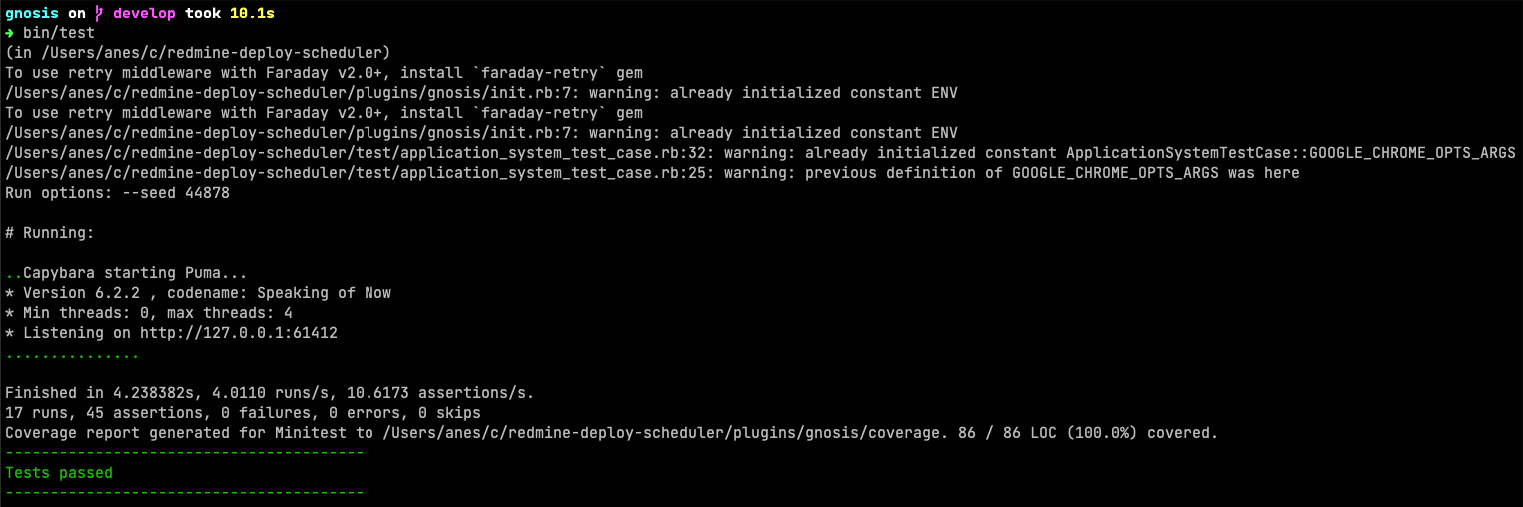
\includegraphics[width=0.75\textwidth]{images/misc/simplecov_terminal_output.png}
    \caption[Ein Screenshot des Terminal Outputs von SimpleCov]{SimpleCov Terminal Output}
    \label{fig:simplecov_terminal_output}
\end{figure}
SimpleCov generiert auch eine HTML Datei, in welcher die Coverage jeder Zeile genau markiert ist in
rot oder grün, je nachdem, ob es getestet wurde oder nicht. So sieht diese Datei in diesem Fall aus:
\begin{figure}[H]
    \centering
    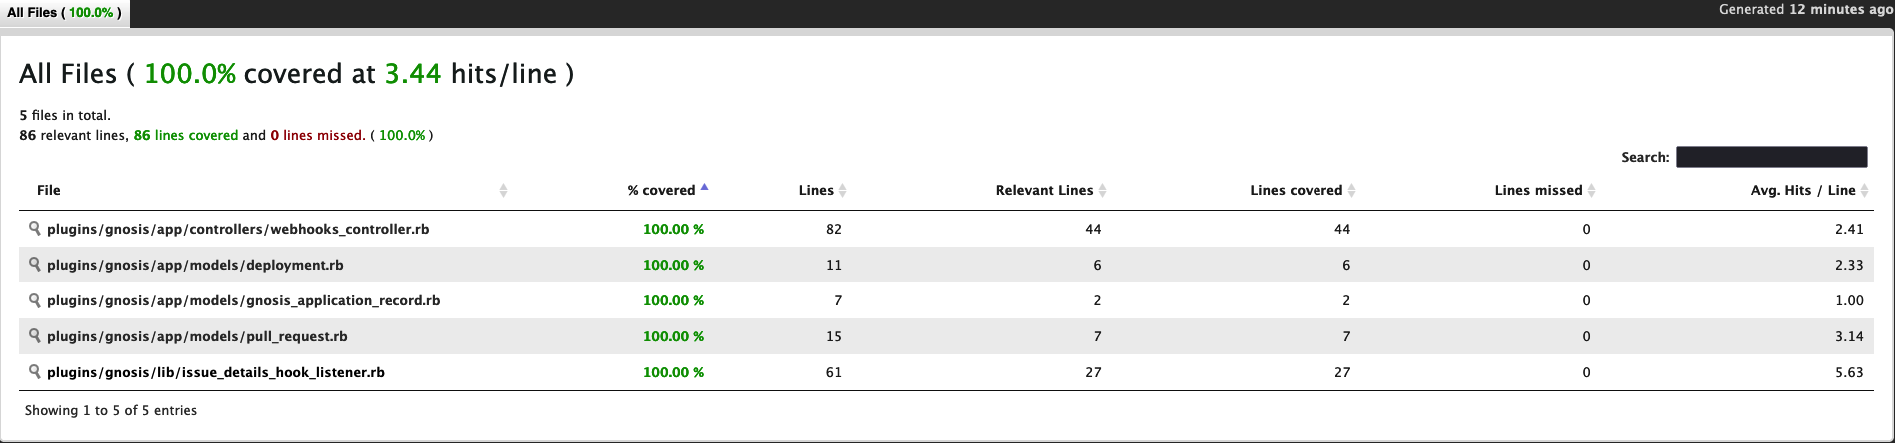
\includegraphics[width=0.75\textwidth]{images/misc/simplecov_html.png}
    \caption[Ein Screenshot des generierten HTML Outputs von SimpleCov]{SimpleCov HTML Output}
    \label{fig:simplecov_html_output}
\end{figure}

\subsubsection{Verscheidene Testarten}
Die Tests befinden sich im \bgmintinline{bash}{test} Verzeichnis. Dort werden diese in verschiedene
Gruppen aufgeteilt, basierend auf der Testart. Die Gruppen sind:
\begin{itemize}
    \item \bgmintinline{bash}{functional} - Funktionale Tests senden Anfragen an die Controller.
    \item \bgmintinline{bash}{unit} - Unittests, welche die einzelnen Klassen und dessen Methoden
    testen.
    \item \bgmintinline{bash}{system} - System Tests klicken sich mit Capybara durch die UI des
    Plugins und testen so die Funktionalität.
\end{itemize}
Die funktionalen Tests wurden für das Testen des \bgmintinline{ruby}{class WebhooksController}
genutzt. Sie schicken Anfragen an den Controller und dessen Funktionen und testen so, ob die richtigen
Objekte basierend auf den Anfragen erstellt werden. \newline
Die Unittests wurden für das Testen der \bgmintinline{ruby}{class Deployment} und 
\bgmintinline{ruby}{class PullRequest} genutzt. Sie testen die einzelnen Methoden dieser Klassen und
prüfen, ob die Objekte richtig manipuliert werden. \newline
Die Systemtests werden für das Testen der UI genutzt. Mithilfe von Capybara wird ein Headless Browser
gestartet, welcher sich durch die UI klickt und so die Funktionalität testet.
\subsection{Style Tests}
Damit der Code \enquote{Clean Code} bleibt, werden Linter verwendet. Diese überprüfen den Code auf Stilfehler,
Sicherheitslücken und andere Fehler. \newline
Da dieses Projekt nur aus Ruby Code besteht, wurde Rubocop in Zusammenarbeit mit Brakeman verwendet. Rubocop
ist dafür zuständig Bugs und Stilfehler zu finden, während Brakeman Sicherheitslücken findet. Diese beiden
Prozesse wurden auch in der CI Pipeline eingebaut, damit der Code immer sauber bleibt:
\begin{figure}[H]
    \centering
    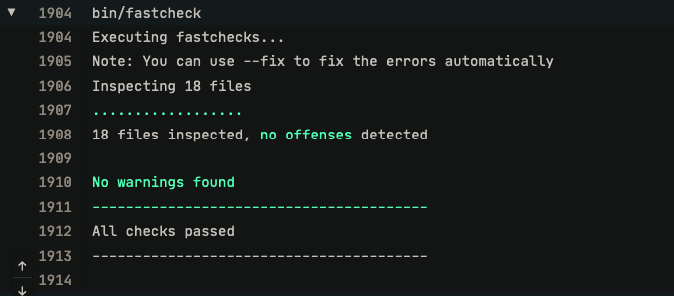
\includegraphics[width=0.75\textwidth]{images/misc/stylecheck_ci.png}
    \caption[Eine Grafik der CI Pipeline mit dem Stylecheck]{CI Pipeline mit Stylecheck}
    \label{fig:ci_pipeline}
\end{figure}

\section{Versionierung}
\label{sec:versioning}
In diesem Kapitel wird die Versionierung von Dokumentation sowie Programmcode beschrieben.
\subsection{Dokumentation}
Die Dokumentation wird mit LaTeX geschrieben und deswegen auch mit Git auf GitHub versioniert. Das
Repository kann unter \url{https://github.com/aneshodza/ipa-documentation} gefunden werden.
\subsubsection{Git-Flow}
Die Versionierung wird nach dem \enquote{Git-Flow} Prinzip gemacht. Das heisst: Es gibt einen main sowie
develop Branch. Der main Branch wird nur bei Releases geändert. Der develop Branch wird für die normale
Entwicklung genutzt. Für jedes neue Kapitel wird ein Feature Branch erstellt.
\subsubsection{Releases}
Am Ende jedes Tages wird ein \enquote{Release} erstellt. Damit ist nicht der main release gemeint, da dieser
nur am Ende des Projekts erstellt wird. Diese Releases finden per Git Tag statt. Dabei wird der letzte
Commit eines Tages mit einem Tag markiert. Das sieht wie folgt aus:
\begin{figure}[H]
    \centering
    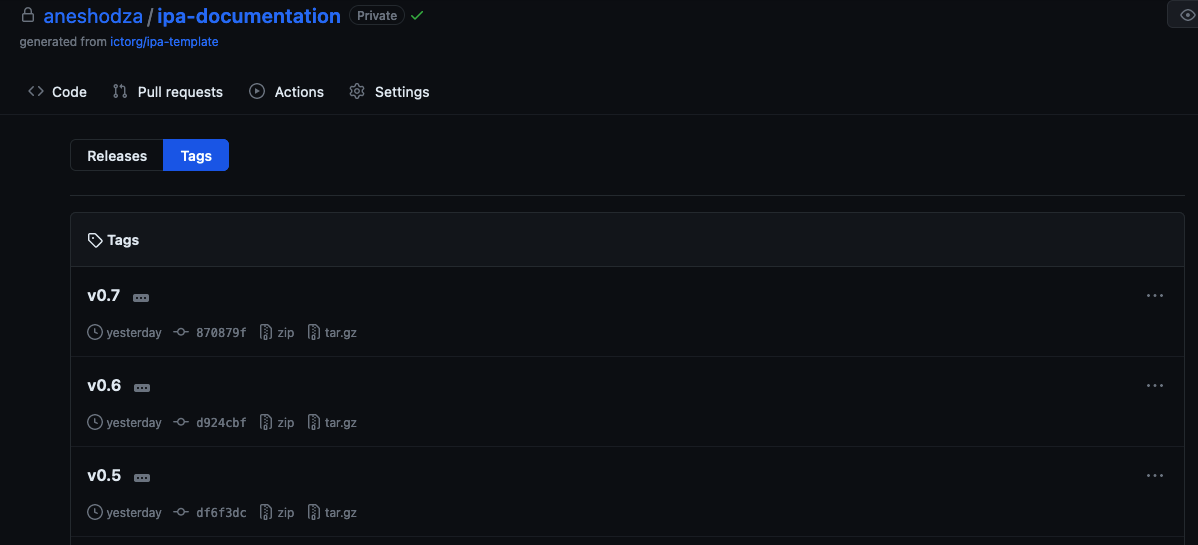
\includegraphics[width=0.75\textwidth]{images/misc/git_tag.png}
    \caption[Ein Screenshot der genutzten Git Tag History für die Versionierung]{Git Tags History}
    \label{fig:git_tag}
\end{figure}

\subsection{Programm}
Der Programmcode wird auch mit Git auf GitHub versioniert. Das Repository kann unter
\url{https://github.com/aneshodza/gnosis} gefunden werden.
\subsubsection{Git-Flow}
Die Versionierung dieses Repositorys wird auch nach dem \enquote{Git-Flow} Prinzip gemacht. Dabei wird
speziell darauf geachtet, dass alle Commit Messages auf Englisch, imperativ und in der Gegenwartsform
geschrieben sind: 
\begin{figure}[H]
    \centering    
    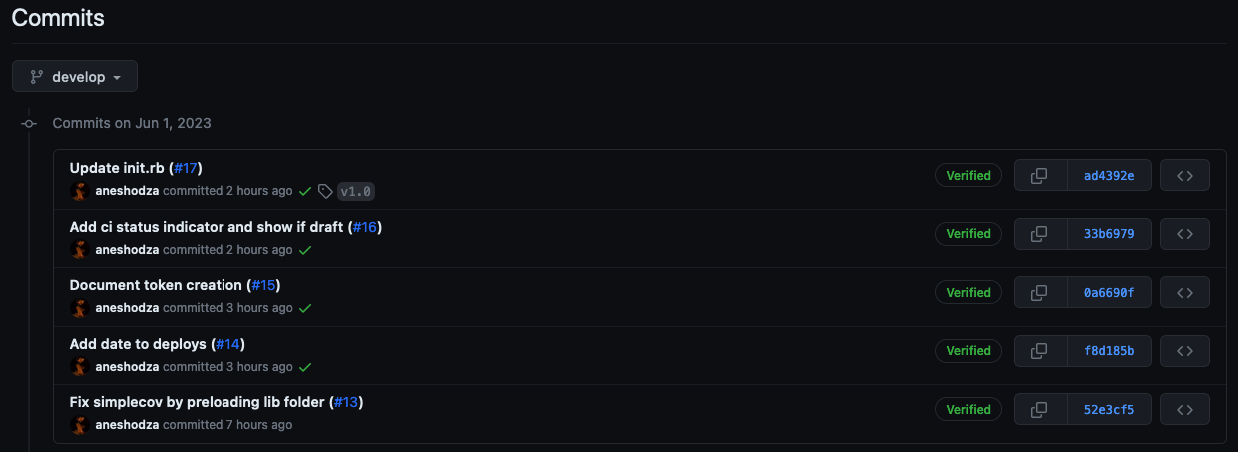
\includegraphics[width=0.75\textwidth]{images/misc/git_commit_message.png}
    \caption[Ein Screenshot der Commit History mit den Commit Messages]{Commit History mit Commit Messages}
    \label{fig:git_commit_message}
\end{figure}
\subsubsection{Selbstkritische Pull Request Reviews}
Bei grösseren Pull Requests wurde ein selbstkritisches Review gemacht. Damit ist gemeint, dass der Code durchgegangen
und auf Fehler überprüft wurde:
\begin{figure}[H]
    \centering
    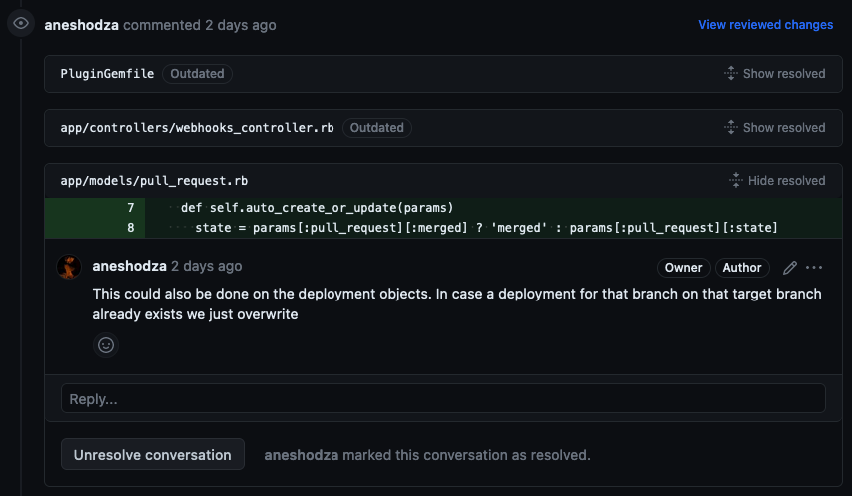
\includegraphics[width=0.75\textwidth]{images/misc/git_pr_review.png}
    \caption[Ein Screenshot eines selbstkritischen Pull Request Reviews]{Selbstkritisches Pull Request Review}
    \label{fig:git_pr_review}
\end{figure}
\subsubsection{Arbeitspakete mit \gls{grün}er CI}
Die Pull Requests entsprechen meistens einem der geplanten Arbeitspaketen und wurden deswegen auch so benannt. Es hat
aber auch einige Pull Requests, welche kein AP waren, da Dinge wie Bugfixes oder Refactorings nicht geplant
werden können. \newline
Dabei wurde auch darauf geachtet, dass der neuste Commit jeder Pull Request grün ist.

\section{Kopplung vom Hauptprogramm}
Eine Anforderung an das Plugin war, dass es möglichst vom Redmine abgekoppelt ist. Das heisst, dass die
Redmine Instanz nicht angepasst werden muss, damit das Plugin funktioniert, sowie, dass das Plugin möglichst
wenig Brücken zu Redmine schlägt. \newline
Damit das Plugin funktioniert, muss Redmine gar nicht angepasst werden, wie in der CI sichtbar. Dort wird
das Plugin einfach installiert und es funktioniert. Auch die Brücken zu Redmine sind sehr klein. Das einzige,
was von Redmine genutzt wird, ist das Issue Objekt. Dieses wird aber nur gelesen und nicht verändert.

\section{Reife der Rails Lösung}
Eine der Kriterien ist die Reife der Rails Lösung, also ob das Produkt in der Produktionsumgebung
eingesetzt werden kann. \newline
Da es eine Test Coverage von 100\% hat, sowie auch problemlos mit der neusten Redmine Version funktioniert,
kann es in der Produktionsumgebung eingesetzt werden. Und falls wenige Sachen ausgebessert werden müssten,
wie zum Beispiel das Handling bei History-Veränderungen, ist das sehr schnell erledigt. Die Codebase ist
sauber und deswegen einfach zu erklären und warten. \newline
Plan B für SemaphoreCI fügte noch eine weitere Schicht Sicherheit hinzu, indem es dem Nutzer garantiert,
dass die richtigen Pull Requests mit Deployments befüllt wurden.
